\label{singlephasedet}

\subsection{DUNE detector plans}

The far detector for the DUNE collaboration will be a series of four liquid argon time projection chambers (TPC), each in a cryostat that holds a fiducial/active/total LAr mass of 10.0/13.3/16.9 kt. The TPCs will be instrumented with photon detection. It is planned that the first 10 kt detector will be ready for installation in the 2021 timeframe. 
The design for the first 10~kt detector is a wire plane based TPC with cold electronics readout. Designs of this style are are referred to as single-phase detectors as the charge generation, drift, and detection all occurs in the liquid argon phase. 
This style TPC features no charge amplification before collection, thereby making a very precise charge measurement possible. 
To achieve DUNE's goals, a detector much larger than ICARUS, the largest LAr TPC detector built to date, is needed. The former long baseline neutrino experiment (LBNE) was developing a scalable far detector design shown in Figure \ref{fig:fardet-overview} that would scale-up LAr TPC technology by roughly a factor of 40 compared to the ICARUS T600 detector. To achieve this scale-up, a number of novel design elements need to be employed. A membrane cryostat typical for the liquefied natural gas industry will be used instead of a conventional evacuated cryostat. The wire planes or anode plane assemblies (APAs) will be factory-built as planar modules that are then installed into the cryostat. The modular nature of the APAs allow the size of the detector to be scaled up to at least 40 kt fiducial mass. Both the analog and digital electronics will be mounted on the wire planes inside the cryostat in order to reduce the electronic noise, to avoid transporting analog signals large distances, and to reduce the number of cables that penetrate the cryostat. The scintillation photon detectors will employ light collection paddles to reduce the required photo-cathode area and thereby cost. 
Many of the aspects of the design are being tested in a small scale prototype at Fermilab but given the very large scale of the detector elements a full-scale test is critical. 
Since the recent formation of the new DUNE collaboration a combined detector design team is emerging. 
Ideas from this new collaboration have the potential to modify the detector design for the additional three far detector modules
which are foreseen for DUNE.
The detector design described here is the LBNE detector design chosen by the DUNE collaboration for the first 10~kt 
detector module and also adopted as the basis for the CERN prototype detector.

\begin{figure}[!htb]
\centering
\begin{minipage}[b]{1.0\textwidth}
\begin{center}
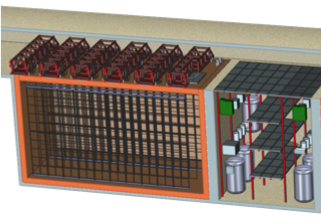
\includegraphics[width=.75\textwidth]{figures/fardet-3D.png}
%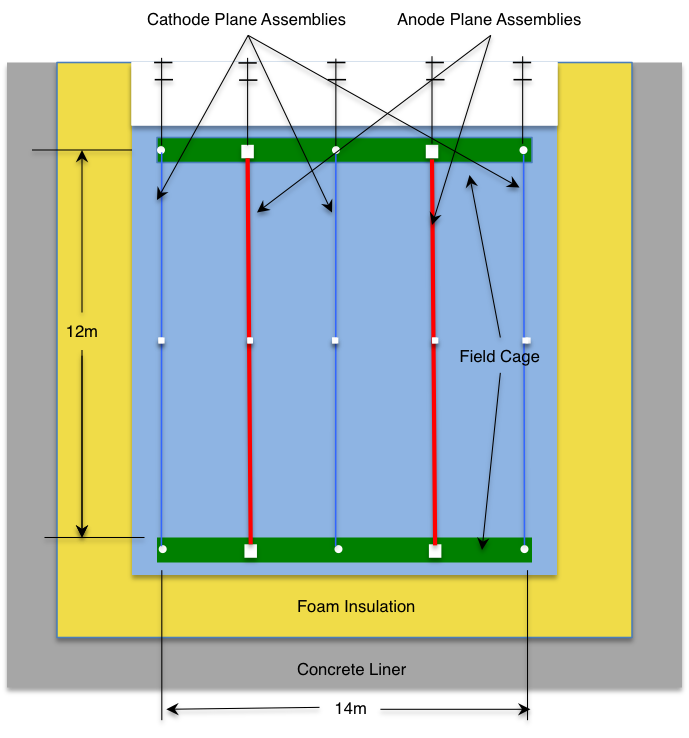
\includegraphics[width=0.7\textwidth]{EndView-sketch.png}
\end{center}
\end{minipage}
\caption{\small 3D model of the design for the first DUNE single-phase detector. Shown is a 5~kt fiducial volume detector which would need to be lengthened for the 10~kt design. The present DUNE plan calls for the construction of four 10~kt detectors. }
\label{fig:fardet-overview} 
\end{figure}

The engineering goals of the DUNE detector test can be broken into five broad categories: 
\begin{enumerate}
	\item TPC performance, mechanical and electrical verification, 
	\item photon detection light yield verification,
	\item calibration strategy verification,
	\item argon contamination mitigation verification, 
	\item production and installation procedure verification
\end{enumerate}

	 The goals related to mechanical testing are to test the integrity of the detector. In the current design, each APA measures 2.3 m by 6.0 m and includes 2560 wires and associated readout channels. Given the complexity of these assemblies, a test where the detector can be thermally cycled and tested under operating conditions is highly advised prior to mass production. The mechanical support of the APAs can be tested to verify that the mechanical design is reliable and will accommodate any necessary motion between the large wire planes. The impact of vibration isolation between the cryostat roof and the detector can also be tested. Finally a potential improvement in the cryostat design is the possibility to move the pumps external to the main cryostat. This will reduce any mechanical coupling to the detector and also greatly improve both reliability and ease of repair. \\

	 
	 The electrical testing goals are to insure that the high voltage design is robust and that the required low electronic noise level can be achieved. As the detector scale increases so does the capacitance and the stored energy in the device. The design of the field cage and high voltage cathode planes needs to be such that HV discharge is unlikely and that if the event occurs no damage to the detector or cryostat results. The grounding and shielding of large detectors is also critical for low noise operation. By testing the full scale elements one insures that the grounding plan is fully developed and effective. Large scale tests of the resulting design will verify the electrical model of the detector. \\

	 Research at Fermilab utilizing the Materials Test Stand has shown that electronegative contamination to the ultra-pure argon from all materials tested is negligible if the material is under the liquid argon. This implies that the dominant source of contamination originates from the gas ullage region and in the room temperature connections to the detector. Careful design of the ullage region to insure that all surfaces and feedthroughs are cold is expected to greatly reduce the sources of contamination over what exists in present detectors. 
	 
\subsection{CERN prototype detector}

%\subsubsection{Overview of the CERN Single-Phase test Detector}


This section presents the design details of a single-phase prototype detector which is based on the development of the LBNE collaboration. 
The DUNE detector design is very modular and the CERN prototype detector will be constructed from modular components of exactly the same design.

\begin{figure}[htb]
\centering
\begin{minipage}[b]{1.0\textwidth}
\begin{center}
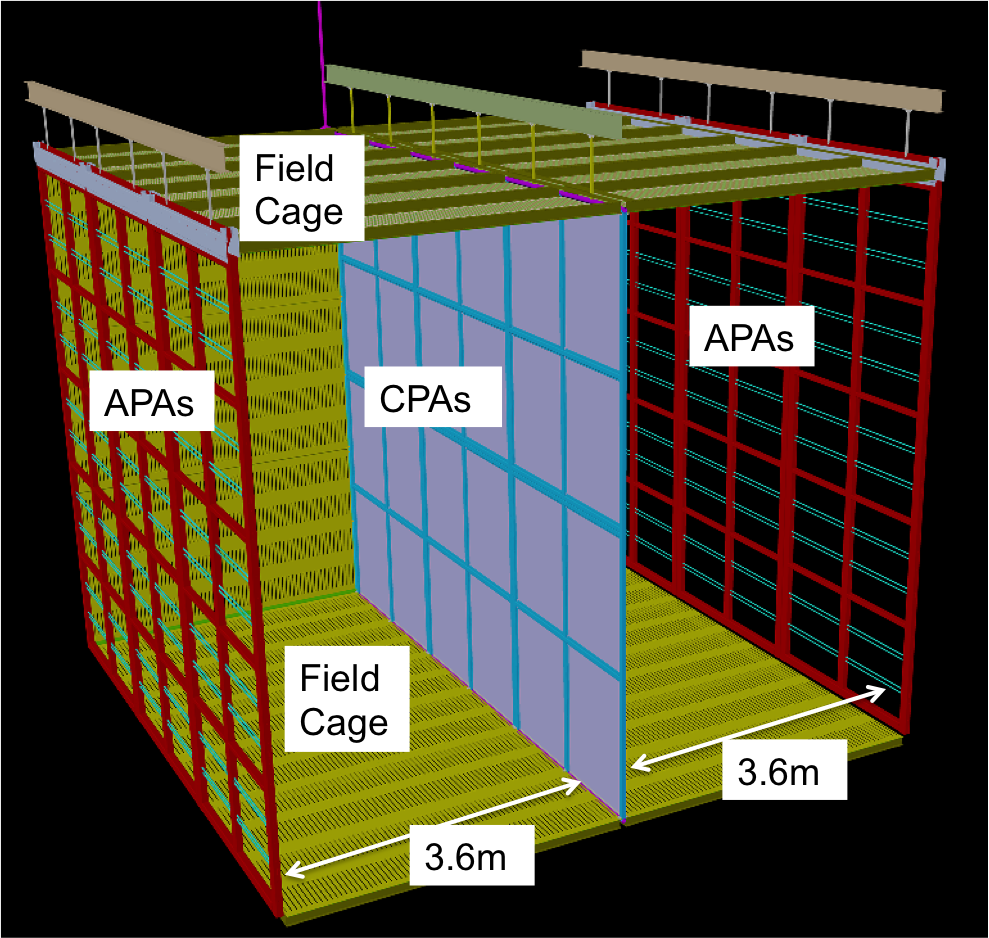
\includegraphics[width=0.40\textwidth]{figures/CERN_single_TPC}
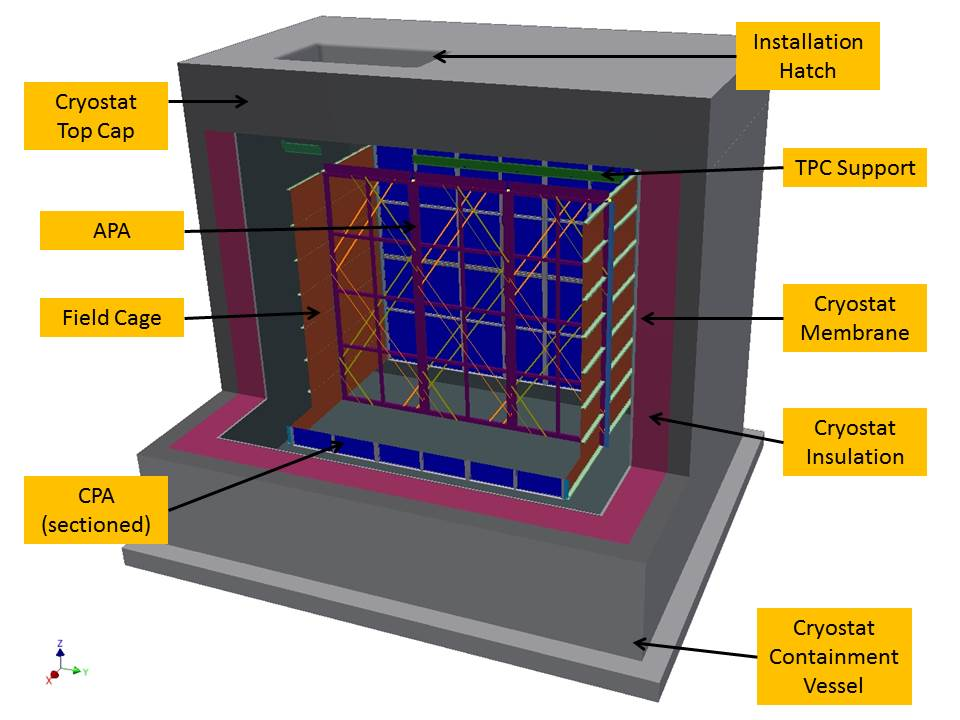
\includegraphics[width=.59\textwidth]{figures/TPC-3D-section.jpg}
\end{center}
\end{minipage}
\caption{\small 3D model of the CERN single-phase detector TPC (left) and inserted in the cryostat (right).}
\label{fig:CERNdet-overview}
\end{figure}

The TPC consists of alternating anode plane assemblies (APAs) and cathode plane assemblies (CPAs), with field-cage panels enclosing the four open sides between the anode and cathode planes.  Figure  \ref{fig:CERNdet-overview} shows a sectioned view for the planned TPC inside the cryostat at CERN.  A uniform electric field is created in the volume between the anode and cathode planes. A charged particle traversing this volume leaves a trail of ionization. The electrons drift toward the anode plane, which is constructed from multiple layers of sense wires, inducing electric current signals in the front-end electronic circuits connected to the wires.

The TPC will be assembled from elements that are of the same size and materials as those planned for the first DUNE far detector module.  

The overall size of the TPC has been determined based on the desired particle containment in order to address the required physics measurements (see section \ref{detbeamtest}). The TPC will have a 3-APA wide active volume and consist of two drift volume with a drift length of 3.6~m each (see figure \ref{fig:CERNdet-overview}).  
The APAs have an active (total) area measuring 2.29 m (2.32 m) wide and 6.0 m (6.2 m) high. The combination of the three APAs determines the overall TPC length to be 7.3m. There will be a cathode plane (CPA) in the center between the two rows of APAs.  
The overall width of the TPC will be determined by a combination of the drift distances along with the thickness of the APAs
and amounts to 7.4~m.  
The overall height of the TPC is determined by the height of the APA which is 6.4m.  The TPC dimensions are summarized in 
table~\ref{table:TPC-dim}.
%
The minimum internal size of the cryostat is also indicated in table \ref{table:TPC-dim} and was determined by adding the necessary mechanical and electrical clearances to the computed size of the TPC.  
 
\begin{table}[h]
\centering
\begin{tabular}{|c|c|}
\hline
\textbf{ Component } & dimensions [m]  \\ \hline \hline
APA  (active) &  $2.29 (wide) \times 6.0 (high)$ \\ \hline
APA  (external) &  $2.32 (wide) \times 6.2 (high)$ \\ \hline
TPC (external)       & $7.3 (long) \times 7.4 (wide) \times 6.4 (high)$  \\ \hline
cryostat (internal) &  $8.9 (long) \times 7.8 (wide) \times 8.1 (high)$  \\ \hline
\end{tabular}
\caption{Dimensions of the single phase prototype detector.}
\label{table:TPC-dim}
\end{table}
 
Along with the APAs and CPAs, the TPC will include a field cage that surrounds the entire assembly to ensure a uniform drift field in the TPC's active volume. 

%This is a series of fiberglass I-beams for the structural elements.  These I-beams will be tiled with large copper sided FR4 panels to create the field cage.  Each panel will be connected with a series of resistors.  The field cage will also be connected to the CPAs through a capacitor assembly.

All of this will be supported by rows of I-beams supported from a mechanical structure above the cryostat.  The hangers for these I-beams will pass through the insulated top cap.  There will be a series of feed-through flanges in the top cap of the cryostat to bring in and take out services for the TPC.  One HV feed-through is foreseen for the CPA row and one signal feed-through for each of the APAs.

The design also foresees the option to have the two APA rows mounted at 2.5~m from the central CPA each.
A reduced drift distance between the APA and CPA represents a deviation from DUNE far detector design but is potentially very
useful in order to lessen the impact of space charge. Due to the operation of the prototype detector on the surface space charge 
 effects are expected to be larger than for underground operation at SURF.
 Depending on the measurement results with a detector which has 3.6~m drift length 
 we are currently considering the possibility for a second test with reduced drift length.
 The cryostat would have to be emptied and the planes shifted to the 2.5~m drift distance.



%The plan is to have the CPA located in the center of the cryostat with APAs on each side near the walls of the cryostat membrane.  The above dimensions preserve the ability to reverse the order of the TPC rows by placing the CPA next to the wall of the cryostat and the APAs in the center.  However, this can only be done with the shorter 2.5m drift distance.  This reversed configuration at the 3.6m drift distance would place the CPAs too close to the membrane and risk high voltage discharge and and thereby possible damage to the membrane.  


% File from Bo Yu on the TPC component design
% Input from Bo and Lee Greenler on the TPC detail design

\subsubsection{Anode Plane Assemblies (APAs)}

% input from Lee Greenler



\begin{figure}[!htb]
\centering
\begin{minipage}[b]{1.0\textwidth}
\begin{center}
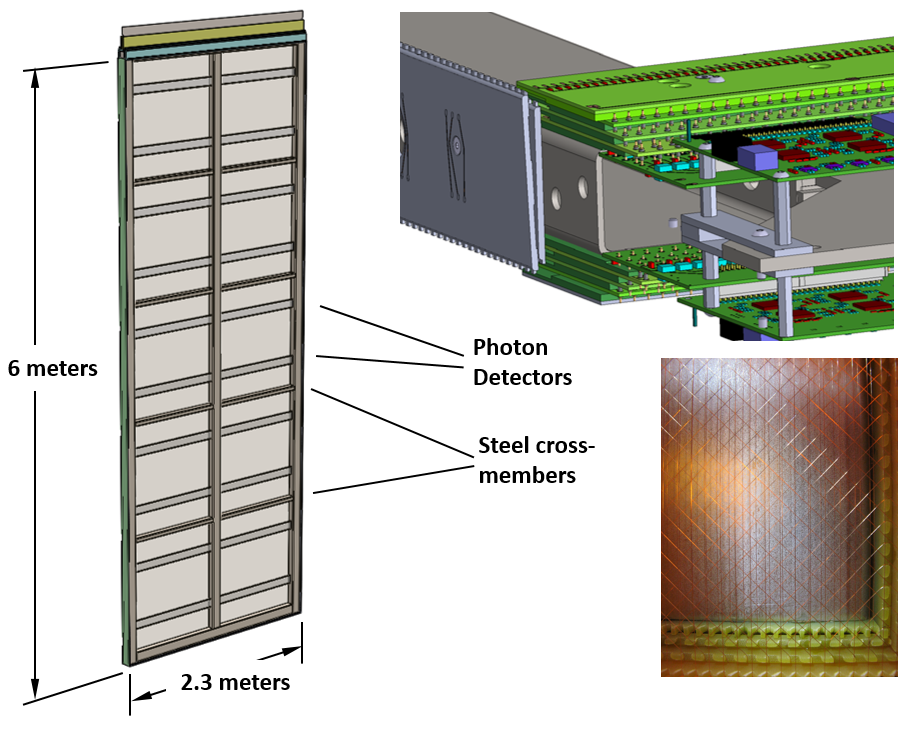
\includegraphics[width=.75\textwidth]{figures/TPC_APA_1}
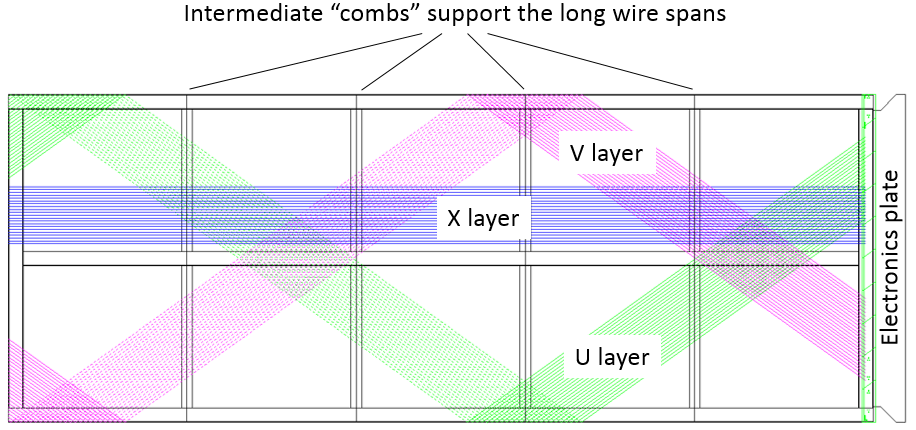
\includegraphics[width=0.75\textwidth]{figures/TPC_APA_2}
\end{center}
\end{minipage}
\caption{Clockwise from left: A full size APA, an APA corner showing the electronics boards, an APA lower corner photo showing wires and edge boards, and a figure showing the wire orientations and the placement of wire aligning combs. }
\label{fig:tpc_apa_overview} 
\end{figure}


Each APA (Figure \ref{fig:tpc_apa_overview}) is instrumented with 3 layers of signal wires, one longitudinal collection plane and two 35.7$^\circ$ angled induction planes with an additional outer grid plane that helps maintain the field. 
The overall dimensions of the active area are 2.3 m wide and 6 m long. The dimension of the wire planes were selected to fit down the Ross shaft at SURF, the future location of the DUNE far detector, be compatible with a standard HiCube transport container, and allow construction from readily available materials.  The wire angle was selected so that a given angled induction wire will not overlay any longitudinal collection wire more than once in order to reduce ambiguities caused by the wrapped wire construction. Partial wire layers are shown in 
Figure ~\ref{fig:tpc_apa_overview} at the bottom.  With a wire pitches of 4.67 mm (diagonal layers) and 4.79 (straight layers), the total number of readout channels in an APA is 2560.
The grid layer is not depicted in Figure ~\ref{fig:tpc_apa_overview} for clarity. The underlying structure of each APA is a framework of rectangular, stainless steel tubing.  The side and bottom edges of the frame are lined with multiple layers of fiberglass circuit boards, notched along the edges to support and locate the wires that cross the APA face. A set of FR4 combs are glued to the APA frame to capture the wires at regular intervals. The front-end electronics boards are mounted at the top end of the frame and protected by a metal enclosure. 


The distance between wire planes is 4.8 mm (3/16 in) matching the standard printed circuit board thickness, and are designed to maintain optimal signal formation. The four wire planes will be electrically biased so that electrons from ionizing-particle tracks completely drift past the first three planes and are collected by the fourth plane. Calculations show that the minimum bias voltages needed to achieve this goal are $V_G$ = -665 V, $V_U$ = -370 V, $V_V$ = 0 V and $V_X$ = 820 V respectively (where G, U, V, and X are the wire-layer labels from outside in, towards the frame).  It is convenient to set one of the wire planes to ground so that the wires can be DC coupled to the front-end readout electronics. In this instance, the V wire plane is set to ground potential to reduce the maximum bias voltages on the other wire planes, and enable the use of lower voltage rated AC coupling capacitors. A grounded mesh plane, located 4.8 mm behind the collection (X) plane, prevents the electric field around this set of wires from being distorted by the metal frame structure and the wires on the opposite side of the frame. It also shields the sensing wires from potential EM interferences from the photon detectors (Fig.~\ref{fig:pd_insertion}) mounted within the frame. The mesh should have a wire pitch less than 2 mm to ensure a uniform electric field while maintaining good optical transparency.


\begin{figure}[t]
  \centering
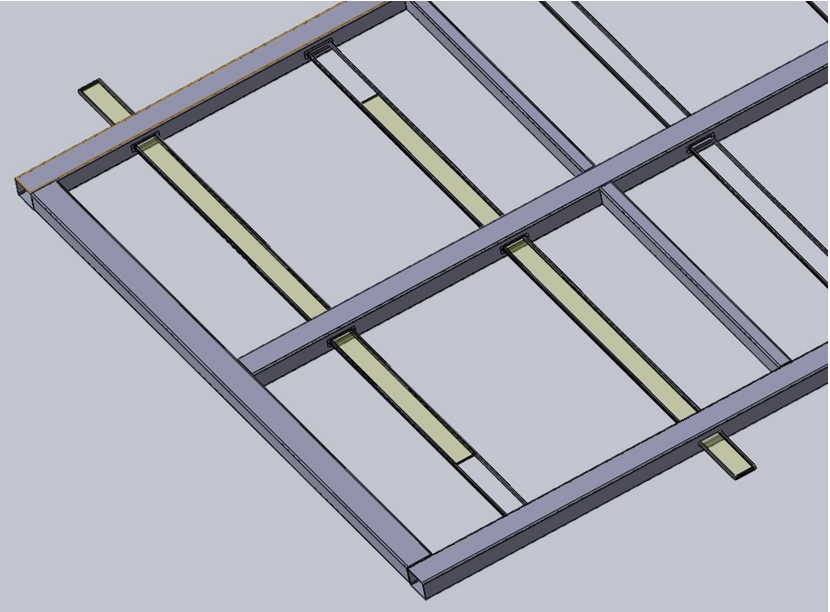
\includegraphics[width=4in]{figures/TPC_APA_3}
  \caption{Photon detectors are mounted within the frame, between the wires on the two sets of four wire layers.  The APA is built so that the photon detectors can be installed through slots in the side of the APA after the APA wires are installed.  The wires that would cross these slots are routed around using copper traces on the edge boards.}
\label{fig:pd_insertion}
\end{figure}


\subsubsection{CPA and Field Cage}

% input from Bo Yu


Each cathode plane (Fig.~\ref{fig:tpc_cpa_1}) is constructed from 6 identical CPA (cathode plane assembly) modules and two sets of end pieces. Each CPA is about half the size of an APA  (2.3m $\times$ 3.1m) for ease of assembly and transport.  The CPA is made of a stainless-steel framework, 
with 4 pieces of thin FR4 sheets mounted in the openings.  A receptacle for the HV feedthrough is attached to the upper corner of a cathode plane toward the roof entrance side to mate with the HV feedthrough in the cryostat ceiling. 

The FR4 sheets on the CPAs are treated with layers of high resistive coating on both sides.  The resistivity of the coating will be chosen such that the surface potential does not deviate significantly with the ionization current from the cosmic rays, and forms a relatively long time constant to dissipate the stored energy on each sheet in case of a high voltage discharge.  This long RC time constant will also reduce the peak current injected into the front-end electronics in a HV discharge.

%Due to the relatively high cosmic ray flux in this surface detector, it is preferable to prevent the scintillation light emitted by a cosmic ray between the cathode and cryostat wall from entering the TPC to reduce false trigger. The opaque cathode surface will service this purpose. 

The high flux of cosmic rays combined with very low drift velocity of positive ions in the liquid argon will result in sizable space charge distortions in the TPC \cite{spacecharge}.  In addition, the positive ions could build up further if the ion motion is slowed or stalled by counter flow in the LAr.  Preliminary CFD analysis \cite{CFD} have shown that solid cathodes in the cryostat result in LAr flow pattern that neither causes excess positive ion buildup, nor degrades the LAr purity.


\begin{figure}[t]
\centering
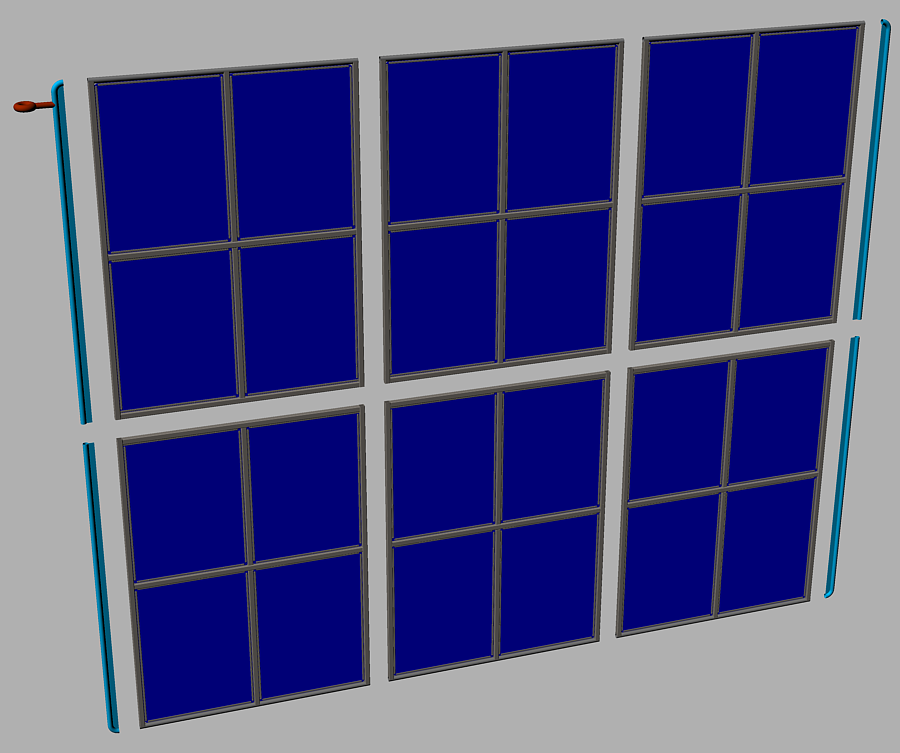
\includegraphics[width=5in]{figures/TPC_CPA_1}
\caption{Exploded view of a cathode plane constructed from 6 CPA modules and 4 end pieces. The facing material on the CPA is highly resistive to minimize the peak energy transfer in case of a HV breakdown.}
\label{fig:tpc_cpa_1}
\end{figure}

To achieve a 500~V/cm drift field over a 3.6~m distance, the bias 
voltage on the cathode plane must reach $-$180~kV. One high voltage power supply (150 -- 200 kV) and one HV feedthrough will be needed for the cathode plane.  The HV feedthroughs are based on the ICARUS design, but modified to further improve the stability at higher voltages. %(Fig.~\ref{fig:tpc_hv_ft}).

%\begin{figure}[hb]
%\centering
%\includegraphics[width=5in]{figures/TPC_HV_FT}  (`figure not found' -- add it then uncomment)
%\caption{Cross section of the HV feedthrough around the end of the grounded shield, and plot of the equi-potential contours between the HV central conductor and the ground shield. The flared end significantly reduces the electric field at the inside of the shield, improving HV stability.}
%\label{fig:tpc_hv_ft}
%\end{figure}



%-%Each pair of facing cathode and anode rows forms an electron-drift region.  A field cage  completely surrounds the four open sides of this region to provide the necessary boundary conditions to ensure a uniform electric field within, unaffected by the presence of the cryostat walls.

\begin{figure}[htb]
\centering
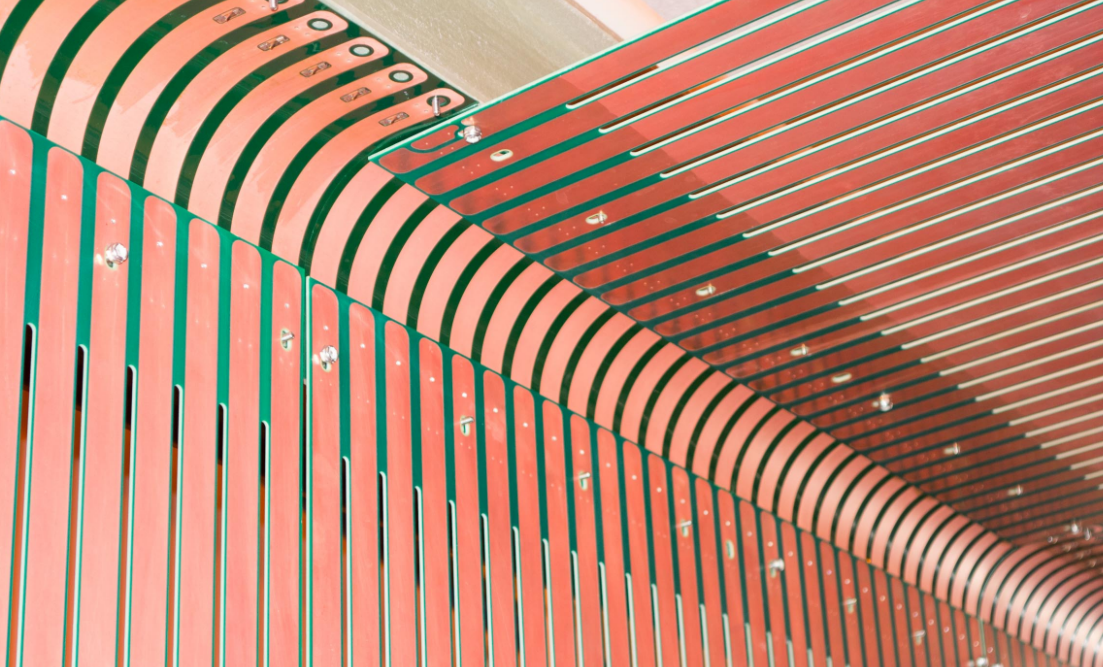
\includegraphics[width=.49\textwidth]{figures/TPC_FCA_1}
%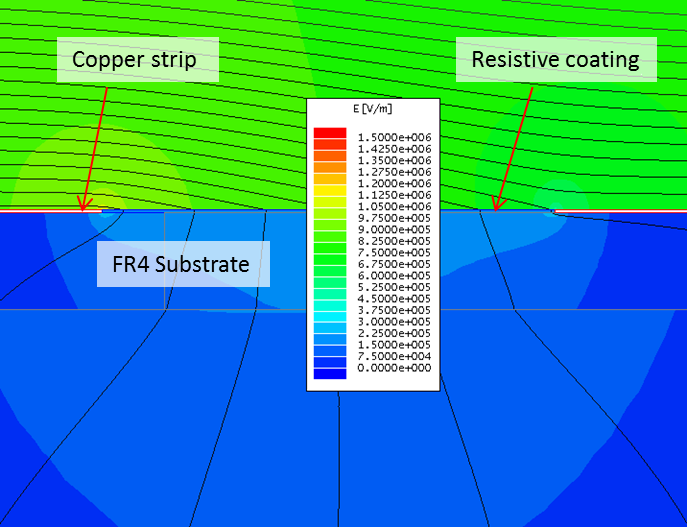
\includegraphics[width=.49\textwidth]{figures/TPC_FCA_2}
\caption{A section of the field cage in the 35ton TPC.}
\label{fig:tpc_fca_1}
\end{figure}    

   

The field cages are constructed using copper-clad FR4 sheets reinforced with fiber glass I-beams to form panels of 2.5~m $\times$ 2.3~m in size for the top and bottom modules, and 2.5~m $\times$ 2~m modules for the sides.  Parallel copper strips are etched or machined on the FR4 sheets.  Strips are biased at appropriate voltages through a resistive divider network. These strips will create a linear electric-potential gradient in the LAr, ensuring a uniform drift field in the TPC's active volume. 
 
%Since the field cage completely encloses the TPC drift region on four (of six) sides, with the remaining two sides blocked by the solid cathodes, the FR4 sheets must  be frequently perforated to allow natural convection of the liquid argon.  The ``transparency'' of the perforation will be determined by a detailed LAr computerized fluid dynamic (CFD) study.

The left of Figure~\ref{fig:tpc_fca_1} shows a section of the field cage in the 35ton TPC as it was being assembled.  The 35ton TPC test results will inform us whether we should improve upon the current design, or consider alternate designs.
% change the design concept all together for this and future detectors.  
%One area of concern with the current field cage design is that the electric field at the edges of the copper strips is still quite high due to the thinness of the copper.  
%One possible remedy is to cover the entire surface of the field cage with a high resistive coating.  The resistivity between strips due to this coating must be kept many orders of magnitudes higher than the divider resistance to avoid distortion to the drift field.  Figure~\ref{fig:tpc_fca_1} (Right-Panel) shows an FEA simulation of such a configuration.

In the event of HV discharge on the cathode or the field cage, the voltage differential between neighboring field cage strips near the discharge electrode will be very high for a brief moment.  This over voltage condition could cause damage to the field cage electrode and the resistors installed between strips.  To minimize such risk, varistors or gas discharge tubes (GDT) will be installed between the field cage strips in parallel with the resistors to prevent excess voltage transient between the electrodes. 

In order to test the installation concept of the far detector, the top and bottom field cage modules will be attached to the mating CPA through hinges.  This combined assembly will be installed into the cryostat and the field cage module opens to connect the CPA and the APA both mechanically and electrically. 








\subsubsection{Photon Detection System}




The ELBNF far detector will utilize liquid argon scintillation light to determine the prompt event time of beam-driven and non-beam events. While the TPC will have a far superior spatial resolution compared to a photon detection system, the drift time for TPC events is on the order of milliseconds. The beam clock will give much better timing resolution than this but a photon detection system can determine the start of an event occurring in the TPC volume (or entering the volume) to about 6~ns, which will be useful in determining the t$_0$ of cosmic ray events, events from radiological decays, and corrections to energy loss of the drifting electrons which in turn improves the particle identification capability of the TPC

A charged particle passing through liquid argon will produce about 40,000 128~nm photons per MeV of deposited energy in the absence of electric fields. At higher electric fields this will be reduced due to reduced recombination, but at 500 V/cm the yield is still about 20,000 photons per MeV. Roughly 1/3 of the photons are prompt 2-6~ns and 2/3 are generated with a delay of 1100-1600~ns. LAr is transparent to the 128~nm VUV photons. At this wavelength, however, the Rayleigh scattering cross-section is large leading to a relatively short Rayleigh scattering length of the order of 55 to 63 ~cm and an absorption length around 200 cm. The relatively large light yield makes the scintillation process an excellent candidate for determination of t$_0$ for non-beam related events. Detection of the scintillation light may also be helpful in background rejection and improving the particle identification.

Several prototypes of photon detection systems have been developed by the LBNE, now ELBNF, photon detector group over the past few years. There are currently three prototypes under consideration for use in the ELBNF far detector, a baseline design along with two alternate designs. A decision on the design to be deployed in the CERN test will be made in late 2015. The CERN neutrino platform ELBNF test would provide the first full scale test of the ELBNF photon detector completely integrated into a full scale TPC anode plane assembly. 

The present reference design for the photon detection system is based on acrylic bars that are 200 cm long and 7.63 cm wide, which are coated with a layer of of the wavelength shifter (WLS)tetraphenyl-butadiene (TPB). The wavelength shifter converts VUV (128 nm) scintillation photons striking it to 430 nm photons inside the bar, with an efficiency of ~50\% of converting a VUV to an optical photon.  A fraction of the wavelength-shifted optical photons are propagated through internal reflection to the bar's end where they are detected by SiPMs whose quantum efficiency (QE) is well matched to the 430 nm wavelength-shifted photons. All PD prototypes are currently using SensL MicroFB-6K-35-SMT 6 mm by 6 mm devices. 

A full 6 m long APA will be divided into 5 bays with 2 PD modules (paddles) instrumenting each bay. The paddles will be inserted into the frames after the TPC wires have been wrapped around the frames allowing  final assembly at the CERN test location. Two alternative designs are also under consideration. 


One alternate design targets increasing the geometrical acceptance of the photon detectors by using large acrylic TPB coated plates with imbedded WLS fibers for readout. In this design the number of required SiPMs and readout channels per unit detector area covered with photon detection panels would be significantly reduced to keep the overall cost for the photon detection system at or below the present design while at the same time increasing the geometrical acceptance. This prototype consists of a TPB-coated acrylic panel embedded with an S-shaped wavelength shifting fiber. The fiber is read out by two SiPMs, which are coupled to either end of the fiber and serves to transport the light over long distances with minimal attenuation. The double-ended fiber readout has the added benefit to provide some position dependence to the light generation along the panel by comparing relative signal sizes and arrival times in the two SiPMs. 



The third design under consideration was motivated by increasing the attenuation length of the PD paddles and allowing collection of 400 nm photons coming from anywhere in the active volume of the TPC.  The fiber-bundle design is based on a thin TPB coated acrylic radiator located in front of a close packed array of WLS fibers. This concept is designed so that roughly half of the photons converted in the radiator are incident on the bundle of fibers, the wavelength shifting fibers are Y11 UV/blue with a 4\% capture probability. The fibers are then read out using SiPMs at one end. The Y11  Kuraray fibers have mean absorption and emission wavelengths of about 440 nm and 480 nm respectively.  The attenuation length of the Y11 fibers is given to be greater than 3.5 m at the mean emission wavelength, which will allow production of full-scale (2 m length) photon detector paddles.

The PD system tested at the CERN neutrino platform will be based on the technology selected later this year. The technology selection process will be based on a series of tests planned for the next 6 months utilizing large research cryostats at Fermilab and Colorado State University. The primary metric used for comparison between the three technologies will be photon yield per unit cost. In addition to this metric photon detection threshold and reliability will also serve as inputs to the final decision. A technical panel will be assembled to make an unbiased decision. 

Once the technology has been chosen the PD group will focus on optimizing the selected design with the goal of procurement and assembly taking place in late FY 2016 and early FY 2016. The photon detector paddles will then be tested and shipped to CERN in early FY 2017 for installation into the APAs in late FY 2017 in preparation for installation into the test cryostat and operation in 2018. 


\subsubsection{TPC and PDS Readout}
A single APA has 2560 sense wires that need to be readout.  In order to  minimizing the capacitance, the preamplier noise, and the number of penetrations through the cryostat, the front-end (FE) electronics boards of the {\bf TPC electronics} are mounted in the cryostat on one end of the wire frame just outside of the active TPC volume.  A single APA is readout by 20 sets of FE readout boards with each FE reading in 128 wire channel inputs (40 U-view + 40 V-view + 48 X-view) and each FE transmitting 4 outputs through the cryostat to back-end electronics.
 
The present design has a maximum wire length of 7.3~m (induction planes)
with a corresponding capacitance of 164~pF and an expected intrinsic noise of 400 electrons.
The preamplifiers include shaping circuits, and are implemented in 16 channel FE ASICs, which couple directly to 16 channel, 12 bit ADC ASICs operating at 2~MS/s, which include a 1:8 multiplexing stage.
The ADCs are read out by a commercial FPGA, which provides an additional factor of 4 in multiplexing.
This level of multiplexing is low enough for transmitting the entire raw data stream,
while also being high enough that the number of signal lines is actually smaller than the number of the various
power and control lines, and therefore easily manageble by a small number of feedthroughs.
Neither zero suppression nor data compression is implemented at the level of the cold readout electronics.
Not only does this greatly simplify the cold electronics design,
but it also automatically satisfies the requirement that the system be capable of such raw readout.
The FPGAs transmit the data via high-speed (1~Gbps) serial links to the DAQ system.
For the final detector it is expected that a dedicated digital control and data transmission ASIC (COLDATA) will be developed which
replaces the commercial FPGA.
While the COLDATA is well under way, it is not expected to be available in time for the CERN test,
which will instead make use of the proven FPGA technology.
While serious doubts regarding the longevity of commercially-available FPGAs at LAr temperatures strongly argues against
their use in the Far Detector, where reliability over 15-20 years is required,
this is not a concern for the CERN test, where the proven FPGA lifetime of at least a year is adequate.

The front end electronics is organized as a stack of three boards comprising the Cold Mother Board assembly (CMB),
which mounts directly on the APA.
First is the Analog Mother Board, on which are mounted the FE and ADC ASICs.
Second and third are the FPGA and SERDES Mezzanine Boards, themselves mounted on the Analog Mother Board.
Each CMB has eight sets of FE and ADC ASICs and instruments 128 wires.
A Faraday cage (FC) covers the end of the APAs to shield the electronics from ambient noise.
The FC also serves to prevent any Ar gas-bubbles from LAr boiled by the electronics' heat from entering the active TPC volume.
Figure \ref{fig:coldelec} shows a schematic of the cold electronics. 

\begin{figure}[htb]
\centering
\begin{minipage}[b]{1.0\textwidth}
\begin{center}
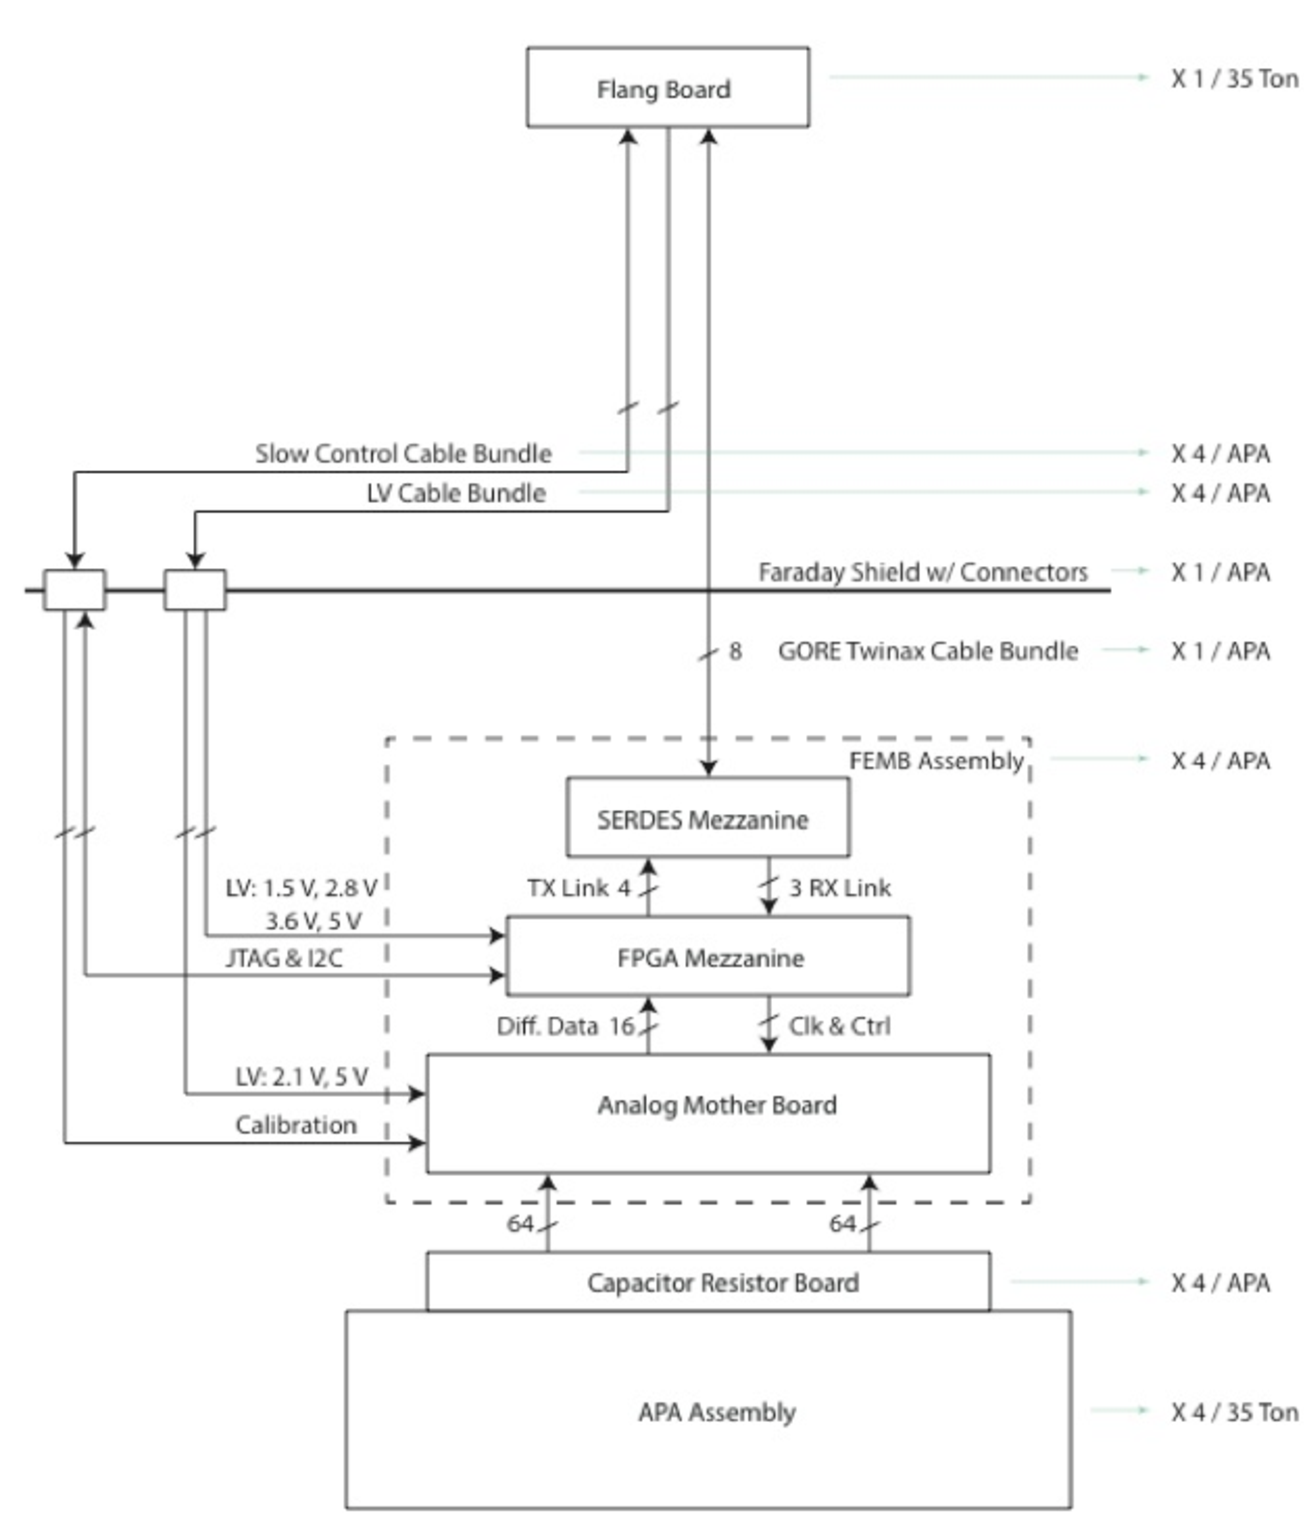
\includegraphics[width=.75\textwidth]{figures/fe-electronics-block-diagram.pdf}
\end{center}
\end{minipage}
\caption{Layout of the TPC cold from end (FE) electronics..}
\label{fig:coldelec}
\end{figure}


Besides the high-speed signal cable, which is a twin-axial cable bundle manufactured by GORE,
there are cable bundles for low-voltage power, wire-bias voltages, and various slow controls and monitoring.
The  cable bundles will be connected through a feedthrough on the roof of the cryostat. 


\begin{figure}[htb]
\centering
\begin{minipage}[b]{1.0\textwidth}
\begin{center}
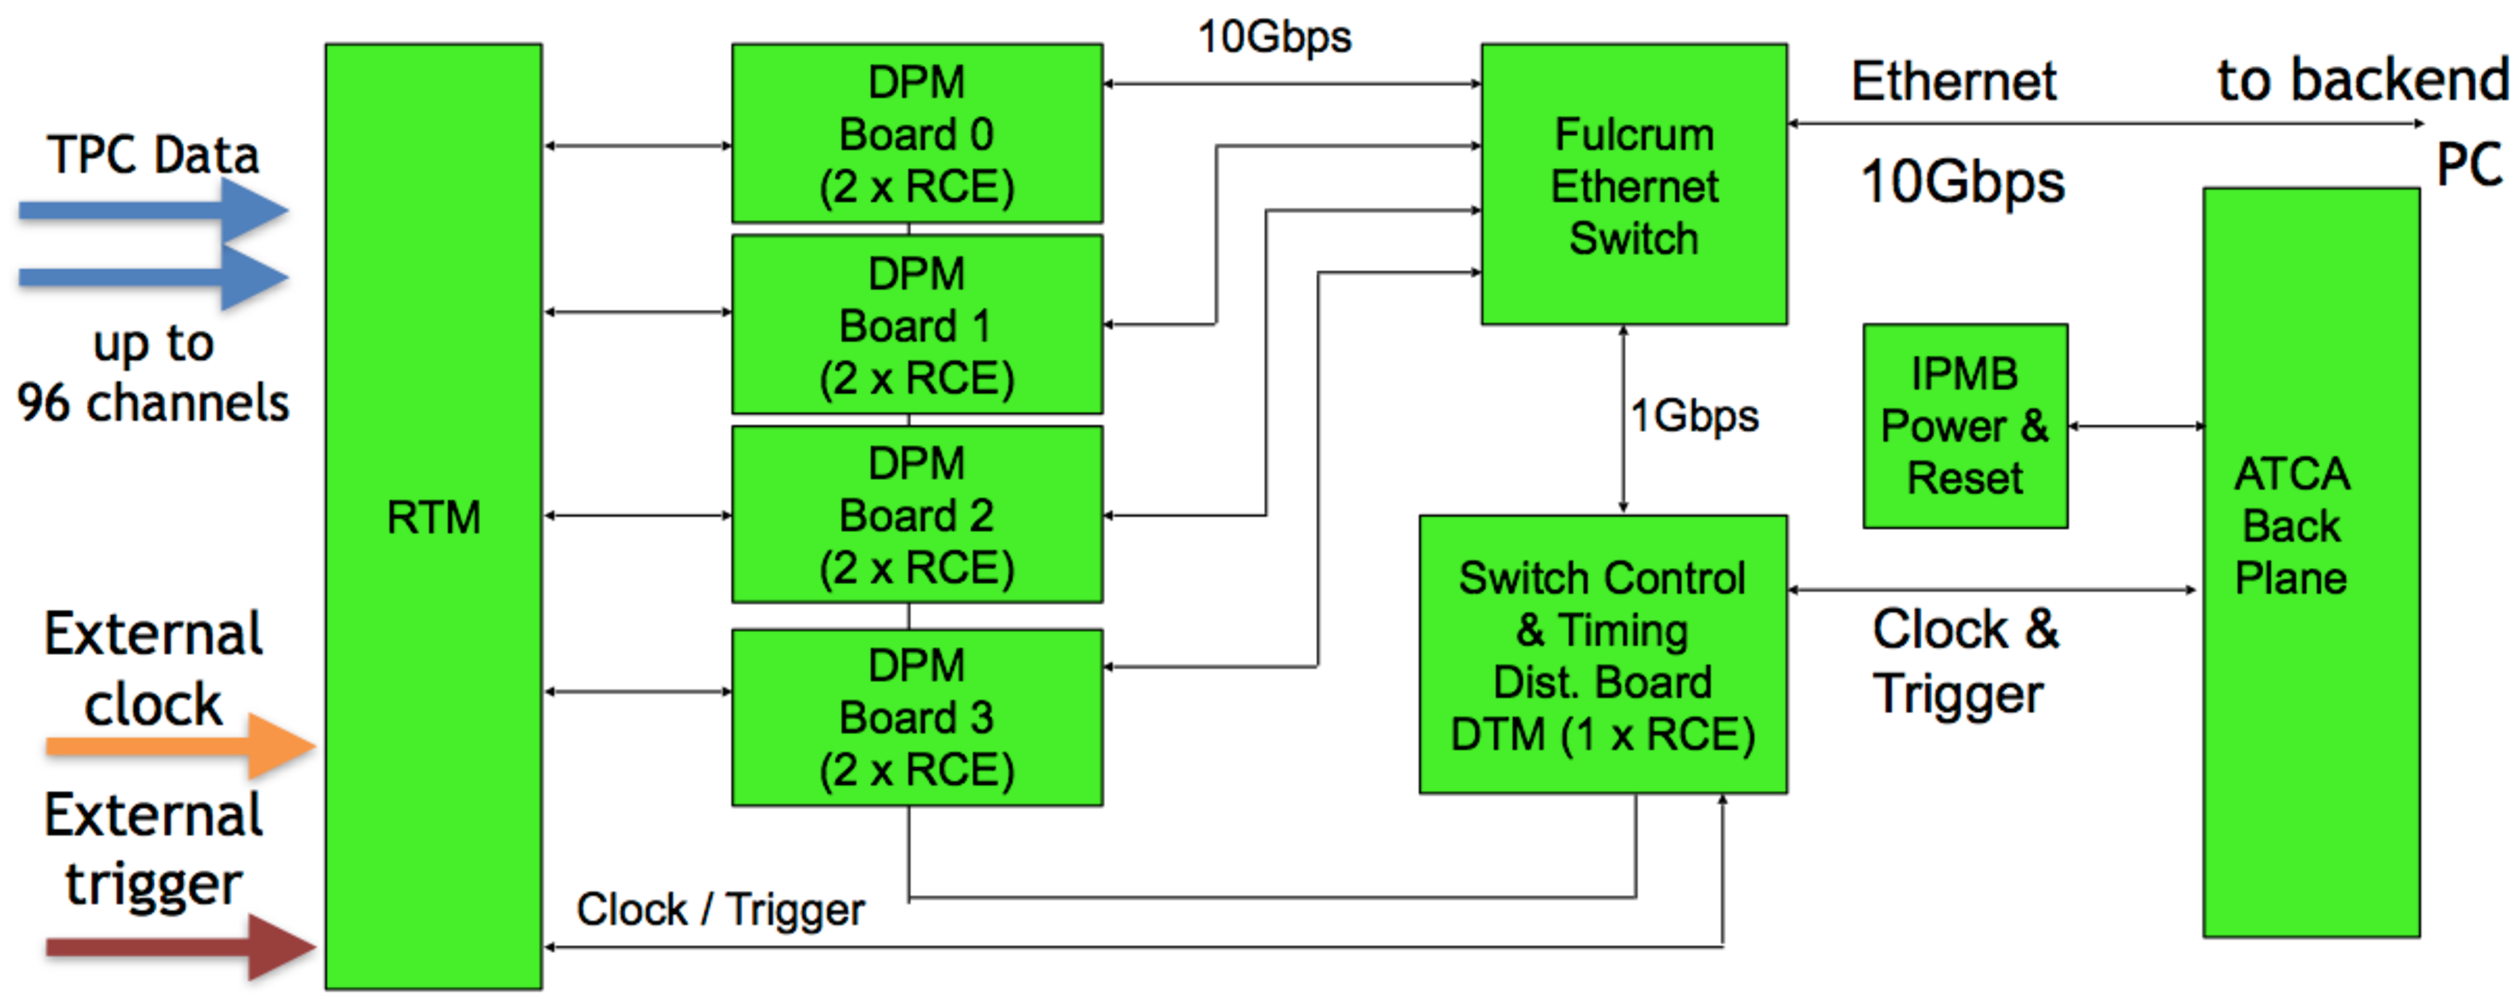
\includegraphics[width=1.0\textwidth]{figures/rce-block.pdf}
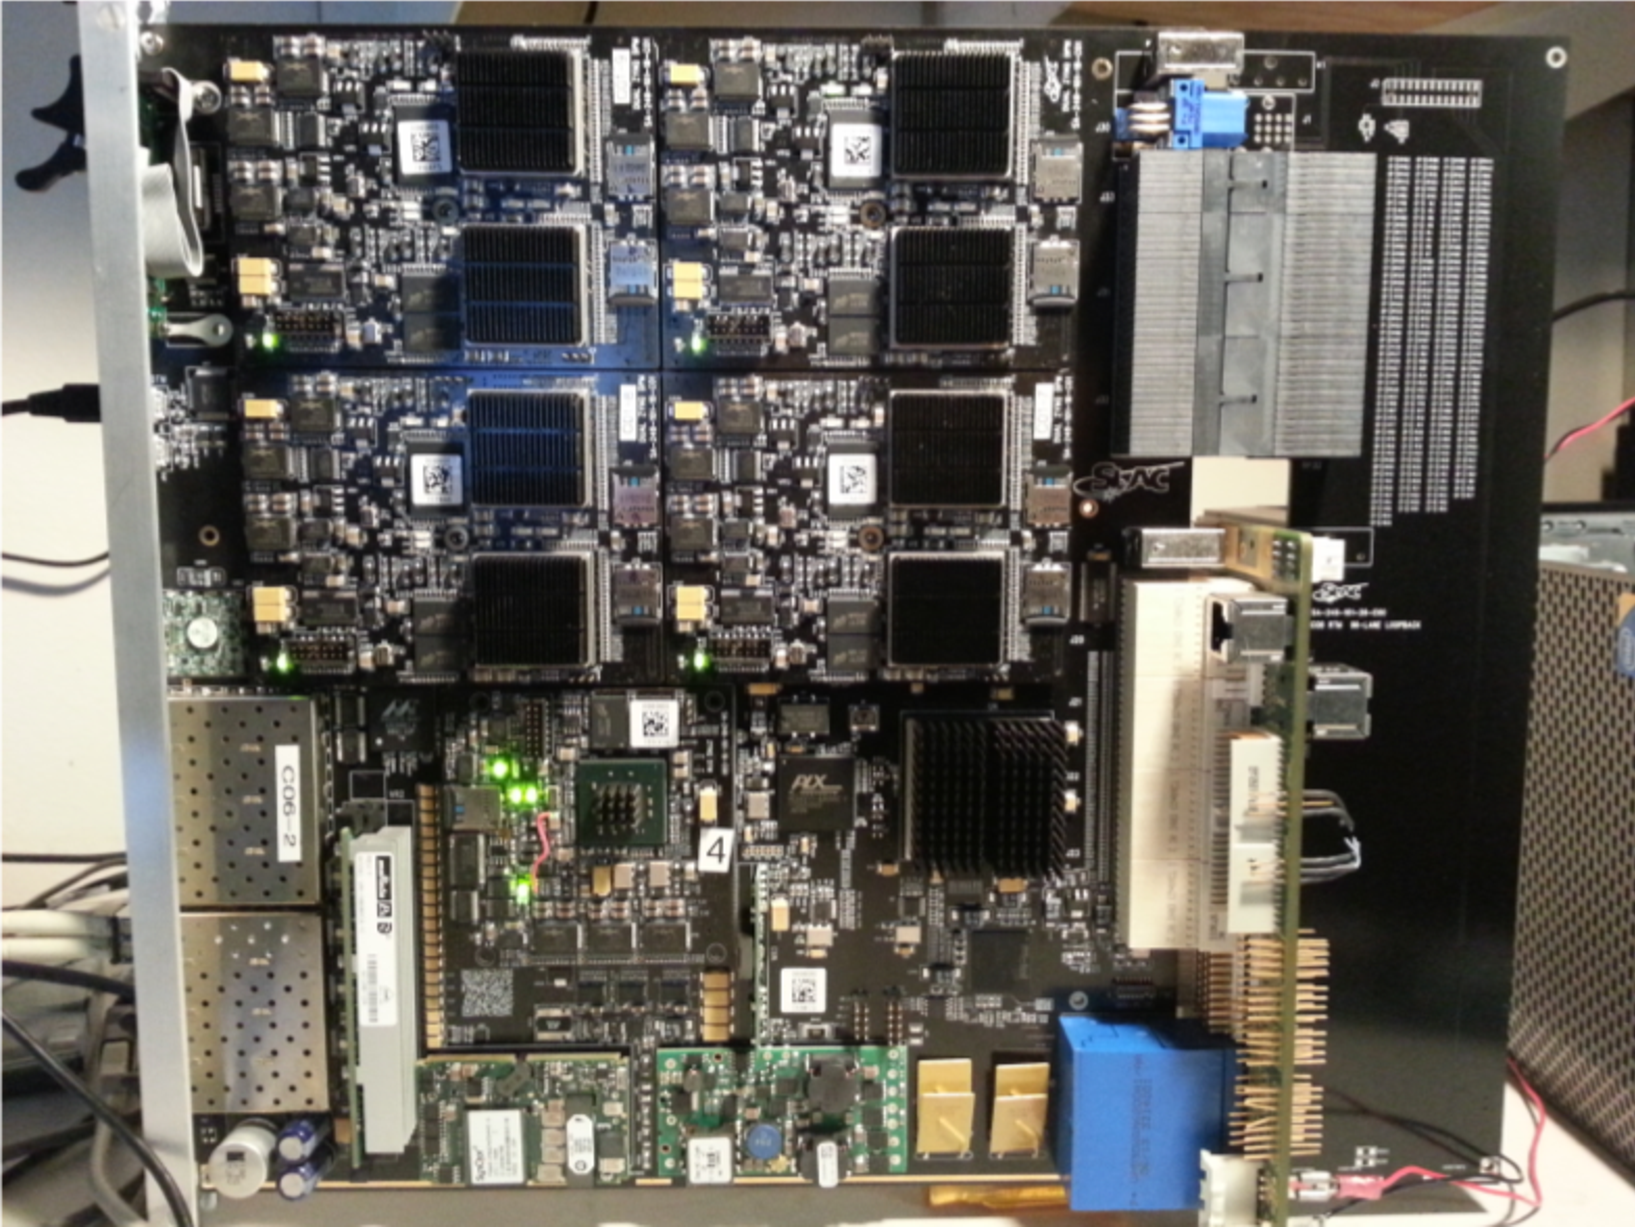
\includegraphics[width=.5\textwidth]{figures/COB-gen3.pdf}
\end{center}
\end{minipage}
\caption{Top: Schematic for the TPC DAQ system. Bottom: The COB (left of the large connectors) and RTM (right).}
\label{fig:rce}
\end{figure}

The primary interface between the TPC front-end electronics (FE) and the DAQ subsystem consists of an ATCA-based system of
RCEs (Reconfigurable Cluster Elements).
The RCE system receives the serialized raw data for the FE, performs zero-suppression on it,
and packetizes and transmits the resulting sparsified data to a back-end data farm for event building and further processing.
Additionally, the RCE system transmits timing and control signals to the FE as well as forwarding configuration data
to them at start-up.     

The RCE system consists of the following components:
a commercial ATCA shelf (2-, 6-, or 14-slot), a Cluster-On-Board (COB) which is the "front board" in ATCA terms,
and a Rear-Transition-Module (RTM) which is the "rear board".
A schematic of the system is shown in Figure \ref{fig:rce}.
The COB is a custom board, developed by SLAC, which holds the processing power of the system.
The COB (see Figure \ref{fig:rce}) consists of 5 bays for holding daughter boards, an onboard 10-GbE switch,
and both 10- and 1-Gb ethernet connections for communications with the back-end system.
Four of the daughter-board bays are for Data Processing Modules (DPM), each of which can hold up to two RCEs.
The RCE is the core procession unit of the system; it is made up of a modern SoC (currently, the Xilinx Zynq-7045)
with multiple high-speed I/O ports (up to 10-Gbps each) and external DRAM and flash memory controllers.
The other bay on the COB contains the Data Transmission Module (DTM) which is responsible
for distributing timing and trigger information to and between the DPMs.  

While the COB hardware is application agnostic, the RTM is application specific.
The RTM provides the mechanical interface between the front-end (or, in our case, the flange electronics)
and the back-end, as well as other external sources such as the timing or trigger systems.
In this case we will use fiber optic connections between the flange and the TPC DAQ using 8 12-channel (full duplex)
CXP connectors on the RTM. 

With the assumption that each cold FE board multiplexes it's 128 wire channels to 4 outputs at 1-Gbps each,
the non-zero suppressed data for 1 APA can be fed into a single COB (containing 8 RCEs).
Each RCE would receive data from 2 FE boards, perform zero-suppression, and send the result to the back-end.  \\


The {\bf PDS front-end electronics} resides outside of the cryostat in
instrumentation racks. A custom module for receiving SiPM signals has
been designed and built. The module also performs signal processing in
the front-end as preprocessing for trigger and DAQ.  The module is
called the SiPM Signal Processor (SSP) and consists of 12 readout
channels packaged in a self-contained 1U module.  Each channel
contains a fully-differential voltage amplifier and a 14-bit, 150-MSPS
analog-to-digital converter (ADC) that digitizes the waveforms
received from the SiPMs. There is no shaping of the signal, since the
SiPM response is slow enough relative to the speed of the digitization
to obtain several digitized samples of the leading edge of the pulse
for the determination of signal timing. Digitized data is processed by
a Xilinx Artix-7 Field-Programmable Gate Array (FPGA).  The use of the
FPGA processing allows for a significant amount of customization of
the SSP operation. \\

%The data streams from the TPC and the PDS will be merged and the concepts are being implemented and tested at the 35t detector.







\subsubsection{DAQ, Slow control and monitoring}
The DAQ will merge data to form events from the LArTPC, 
photon detector and beam detector readouts using the 
artDAQ data acquisition toolkit using a farm of commercial 
computers connected with an Ethernet switch.  ArtDAQ is 
in use on several experiments at Fermilab.  We are using it
on the 35t prototype, so we will have considerable 
experience by the time of the CERN test.  

The data collection for the CERN test will operate in a mode 
similar to that forseen for the underground detectors. In order 
to collect data from non-beam interactions such as proton decay 
candidates or atmospheric neutrinos, data will be continuously
read in to the artDAQ data receiver nodes and processed through
the artDAQ system in quanta corresponding to time intervals fixed
from the time of the beginning of the run.  These are then 
transferred through the switch to a set of event building nodes 
which work in parallel, each node receiving all the data from all 
the detectors for the time intervals it is responsible for processing.
There will be 32 parallel incoming data streams from the LArTPCs
and 16 streams from the photon detectors.  There will be an additional
stream from the trigger board (the same board as built by Penn for
the 35t test will be used) which will receive input of the spill 
gate, warning of extraction, and pattern-unit bits from trigger counters
and other beamline instrumentation such as Cerenkov counters [Which 
section are these described in?, should we refer to them from here?].

Synchronisation across all the input sources is essential in order 
that artDAQ can bring together the data from the input streams correctly for
processing by the event building nodes.  The data receiver nodes will provide
overlap by repeating the data at the boundaries of the time intervals so 
that a particle whose data spans two time intervals can be collected.  
The time synchronisation is provided to the RTM back-module on the LArTPC 
readout crates, to the SSP photon detector readout and to the trigger board from
a GPS based time synchrononisation distribution system originally designed 
for the NOvA experiment.  This system includes functionality to calibrate and 
correct for the cable delays, and to send synchronisation control signals to
the readout at predetermined times.

The event building nodes will select time regions of interest within the time 
intervals they are processing and form these into events to be written to 
disk. The algorithms to select the events may be as simple as looking for 
a trigger bit in the trigger board data stream, or may involve looking 
for self-triggered events in the LArTPC data.  An aggregation task, which 
is part of artDAQ will handle the parallelized event building processes by 
merging the output events into a single stream and writing them to disk.
To avoid oversized output data files, when a predetrmined file size is reached, 
the aggregator will switch to writing to a new file.  The collaboraion 
requests to CERN, data links of sufficient bandwidth to transfer these files 
from the CENF to the CERN data center, and from there to locations 
worldwide for analysis. 

Improved versions of the software systems which are being prototyped at the 
35t test will available for the CERN test including (a) Run control which 
controls and monitors the DAQ processes and allows run starts and stops to
be performed by the operator (b) online monitoring (c) slow control of 
voltages and temperatures being used by the electronics (this may not be 
comprehensive by the time of the CERN protoype, but we plan on prototyping 
the readout of some of the quantities).  The trigger board includes facilities 
for generating calibration pulses and for identifying the event times of 
the calibration events.






